\documentclass[twoside]{book}

% Packages required by doxygen
\usepackage{fixltx2e}
\usepackage{calc}
\usepackage{doxygen}
\usepackage[export]{adjustbox} % also loads graphicx
\usepackage{graphicx}
\usepackage[utf8]{inputenc}
\usepackage{makeidx}
\usepackage{multicol}
\usepackage{multirow}
\PassOptionsToPackage{warn}{textcomp}
\usepackage{textcomp}
\usepackage[nointegrals]{wasysym}
\usepackage[table]{xcolor}

% Font selection
\usepackage[T1]{fontenc}
\usepackage[scaled=.90]{helvet}
\usepackage{courier}
\usepackage{amssymb}
\usepackage{sectsty}
\renewcommand{\familydefault}{\sfdefault}
\allsectionsfont{%
  \fontseries{bc}\selectfont%
  \color{darkgray}%
}
\renewcommand{\DoxyLabelFont}{%
  \fontseries{bc}\selectfont%
  \color{darkgray}%
}
\newcommand{\+}{\discretionary{\mbox{\scriptsize$\hookleftarrow$}}{}{}}

% Page & text layout
\usepackage{geometry}
\geometry{%
  a4paper,%
  top=2.5cm,%
  bottom=2.5cm,%
  left=2.5cm,%
  right=2.5cm%
}
\tolerance=750
\hfuzz=15pt
\hbadness=750
\setlength{\emergencystretch}{15pt}
\setlength{\parindent}{0cm}
\setlength{\parskip}{3ex plus 2ex minus 2ex}
\makeatletter
\renewcommand{\paragraph}{%
  \@startsection{paragraph}{4}{0ex}{-1.0ex}{1.0ex}{%
    \normalfont\normalsize\bfseries\SS@parafont%
  }%
}
\renewcommand{\subparagraph}{%
  \@startsection{subparagraph}{5}{0ex}{-1.0ex}{1.0ex}{%
    \normalfont\normalsize\bfseries\SS@subparafont%
  }%
}
\makeatother

% Headers & footers
\usepackage{fancyhdr}
\pagestyle{fancyplain}
\fancyhead[LE]{\fancyplain{}{\bfseries\thepage}}
\fancyhead[CE]{\fancyplain{}{}}
\fancyhead[RE]{\fancyplain{}{\bfseries\leftmark}}
\fancyhead[LO]{\fancyplain{}{\bfseries\rightmark}}
\fancyhead[CO]{\fancyplain{}{}}
\fancyhead[RO]{\fancyplain{}{\bfseries\thepage}}
\fancyfoot[LE]{\fancyplain{}{}}
\fancyfoot[CE]{\fancyplain{}{}}
\fancyfoot[RE]{\fancyplain{}{\bfseries\scriptsize Generated by Doxygen }}
\fancyfoot[LO]{\fancyplain{}{\bfseries\scriptsize Generated by Doxygen }}
\fancyfoot[CO]{\fancyplain{}{}}
\fancyfoot[RO]{\fancyplain{}{}}
\renewcommand{\footrulewidth}{0.4pt}
\renewcommand{\chaptermark}[1]{%
  \markboth{#1}{}%
}
\renewcommand{\sectionmark}[1]{%
  \markright{\thesection\ #1}%
}

% Indices & bibliography
\usepackage{natbib}
\usepackage[titles]{tocloft}
\setcounter{tocdepth}{3}
\setcounter{secnumdepth}{5}
\makeindex

% Hyperlinks (required, but should be loaded last)
\usepackage{ifpdf}
\ifpdf
  \usepackage[pdftex,pagebackref=true]{hyperref}
\else
  \usepackage[ps2pdf,pagebackref=true]{hyperref}
\fi
\hypersetup{%
  colorlinks=true,%
  linkcolor=blue,%
  citecolor=blue,%
  unicode%
}

% Custom commands
\newcommand{\clearemptydoublepage}{%
  \newpage{\pagestyle{empty}\cleardoublepage}%
}

\usepackage{caption}
\captionsetup{labelsep=space,justification=centering,font={bf},singlelinecheck=off,skip=4pt,position=top}

%===== C O N T E N T S =====

\begin{document}

% Titlepage & ToC
\hypersetup{pageanchor=false,
             bookmarksnumbered=true,
             pdfencoding=unicode
            }
\pagenumbering{alph}
\begin{titlepage}
\vspace*{7cm}
\begin{center}%
{\Large Projeto \\[1ex]\large 1 }\\
\vspace*{1cm}
{\large Generated by Doxygen 1.8.14}\\
\end{center}
\end{titlepage}
\clearemptydoublepage
\pagenumbering{roman}
\tableofcontents
\clearemptydoublepage
\pagenumbering{arabic}
\hypersetup{pageanchor=true}

%--- Begin generated contents ---
\chapter{Hierarchical Index}
\section{Class Hierarchy}
This inheritance list is sorted roughly, but not completely, alphabetically\+:\begin{DoxyCompactList}
\item \contentsline{section}{Point}{\pageref{class_point}}{}
\item \contentsline{section}{Poligono}{\pageref{class_poligono}}{}
\begin{DoxyCompactList}
\item \contentsline{section}{Retangulo}{\pageref{class_retangulo}}{}
\end{DoxyCompactList}
\end{DoxyCompactList}

\chapter{Class Index}
\section{Class List}
Here are the classes, structs, unions and interfaces with brief descriptions\+:\begin{DoxyCompactList}
\item\contentsline{section}{\hyperlink{classMainWindow}{Main\+Window} \\*\hyperlink{classMainWindow}{Main\+Window} recebe e trata os dados recebidos no servidor }{\pageref{classMainWindow}}{}
\end{DoxyCompactList}

\chapter{Class Documentation}
\hypertarget{class_point}{}\section{Point Class Reference}
\label{class_point}\index{Point@{Point}}


The \mbox{\hyperlink{class_point}{Point}} class serve para realizar e manipular pontos de dados do tipo float.  




{\ttfamily \#include $<$point.\+h$>$}

\subsection*{Public Member Functions}
\begin{DoxyCompactItemize}
\item 
void \mbox{\hyperlink{class_point_a428a1676e2fdec6753c42011a1d59d18}{setX}} (float \+\_\+x)
\begin{DoxyCompactList}\small\item\em setX é uma função da classe que serve para setar a variável \+\_\+x do ponto. \end{DoxyCompactList}\item 
void \mbox{\hyperlink{class_point_a9868c4601b0ea0c2d0de20fe41ee0e49}{setY}} (float \+\_\+y)
\begin{DoxyCompactList}\small\item\em setY é uma função da classe que serve para setar a variável \+\_\+y do ponto. \end{DoxyCompactList}\item 
void \mbox{\hyperlink{class_point_ab5385c6d9bfa841e641e4709fc9f14cc}{set\+XY}} (float \+\_\+x, float \+\_\+y)
\begin{DoxyCompactList}\small\item\em set\+XY é uma função da classe que serve para setar, diretamente, as variáveis \+\_\+x e \+\_\+y do ponto. \end{DoxyCompactList}\item 
float \mbox{\hyperlink{class_point_a9aa94b8fd07296e64d304ef3750db113}{getX}} (void)
\begin{DoxyCompactList}\small\item\em getX é uma função da classe que serve para recuperar o valor da variável \+\_\+x do ponto. \end{DoxyCompactList}\item 
float \mbox{\hyperlink{class_point_a2444daa96871c89614510bc4bfcd19ce}{getY}} (void)
\begin{DoxyCompactList}\small\item\em getY é uma função da classe que serve para recuperar o valor da variável \+\_\+y do ponto. \end{DoxyCompactList}\item 
void \mbox{\hyperlink{class_point_a6bcf8fd2524ecc4d5b6c1dc942d541a5}{add}} (\mbox{\hyperlink{class_point}{Point}} p1)
\begin{DoxyCompactList}\small\item\em add é uma função da classe que serve para somar dois pontos. \end{DoxyCompactList}\item 
void \mbox{\hyperlink{class_point_af7d9e533f0030edf4ab28fdc0f12acd4}{sub}} (\mbox{\hyperlink{class_point}{Point}} p1)
\begin{DoxyCompactList}\small\item\em sub é uma função da classe que serve para subtrair dois pontos. \end{DoxyCompactList}\item 
float \mbox{\hyperlink{class_point_abd2618d1f505d9392893273a66e7c9b2}{norma}} ()
\begin{DoxyCompactList}\small\item\em norma é uma função da classe que serve para calcular a norma do ponto. \end{DoxyCompactList}\item 
void \mbox{\hyperlink{class_point_ad9676e36f3444534b609e3c68422239a}{translada}} (float a, float b)
\begin{DoxyCompactList}\small\item\em translada é uma função da classe que serve para transladar um ponto no eixo x em \char`\"{}a\char`\"{} unidades e no eixo y em \char`\"{}b\char`\"{} unidades. \end{DoxyCompactList}\item 
\mbox{\Hypertarget{class_point_a188350fb70e5b297a659a31ab8887ca3}\label{class_point_a188350fb70e5b297a659a31ab8887ca3}} 
void \mbox{\hyperlink{class_point_a188350fb70e5b297a659a31ab8887ca3}{imprime}} (void)
\begin{DoxyCompactList}\small\item\em imprime é uma função da classe que serve para imprimir o ponto na tela. \end{DoxyCompactList}\end{DoxyCompactItemize}


\subsection{Detailed Description}
The \mbox{\hyperlink{class_point}{Point}} class serve para realizar e manipular pontos de dados do tipo float. 

\subsection{Member Function Documentation}
\mbox{\Hypertarget{class_point_a6bcf8fd2524ecc4d5b6c1dc942d541a5}\label{class_point_a6bcf8fd2524ecc4d5b6c1dc942d541a5}} 
\index{Point@{Point}!add@{add}}
\index{add@{add}!Point@{Point}}
\subsubsection{\texorpdfstring{add()}{add()}}
{\footnotesize\ttfamily void Point\+::add (\begin{DoxyParamCaption}\item[{\mbox{\hyperlink{class_point}{Point}}}]{p1 }\end{DoxyParamCaption})}



add é uma função da classe que serve para somar dois pontos. 


\begin{DoxyParams}{Parameters}
{\em p1} & é um ponto inserido pelo usuário. \\
\hline
\end{DoxyParams}
\mbox{\Hypertarget{class_point_a9aa94b8fd07296e64d304ef3750db113}\label{class_point_a9aa94b8fd07296e64d304ef3750db113}} 
\index{Point@{Point}!getX@{getX}}
\index{getX@{getX}!Point@{Point}}
\subsubsection{\texorpdfstring{get\+X()}{getX()}}
{\footnotesize\ttfamily float Point\+::getX (\begin{DoxyParamCaption}\item[{void}]{ }\end{DoxyParamCaption})}



getX é uma função da classe que serve para recuperar o valor da variável \+\_\+x do ponto. 

\begin{DoxyReturn}{Returns}
Valor do \+\_\+x do ponto. 
\end{DoxyReturn}
\mbox{\Hypertarget{class_point_a2444daa96871c89614510bc4bfcd19ce}\label{class_point_a2444daa96871c89614510bc4bfcd19ce}} 
\index{Point@{Point}!getY@{getY}}
\index{getY@{getY}!Point@{Point}}
\subsubsection{\texorpdfstring{get\+Y()}{getY()}}
{\footnotesize\ttfamily float Point\+::getY (\begin{DoxyParamCaption}\item[{void}]{ }\end{DoxyParamCaption})}



getY é uma função da classe que serve para recuperar o valor da variável \+\_\+y do ponto. 

\begin{DoxyReturn}{Returns}
Valor do \+\_\+y do ponto. 
\end{DoxyReturn}
\mbox{\Hypertarget{class_point_abd2618d1f505d9392893273a66e7c9b2}\label{class_point_abd2618d1f505d9392893273a66e7c9b2}} 
\index{Point@{Point}!norma@{norma}}
\index{norma@{norma}!Point@{Point}}
\subsubsection{\texorpdfstring{norma()}{norma()}}
{\footnotesize\ttfamily float Point\+::norma (\begin{DoxyParamCaption}{ }\end{DoxyParamCaption})}



norma é uma função da classe que serve para calcular a norma do ponto. 

\begin{DoxyReturn}{Returns}
Valor calculado da norma. 
\end{DoxyReturn}
\mbox{\Hypertarget{class_point_a428a1676e2fdec6753c42011a1d59d18}\label{class_point_a428a1676e2fdec6753c42011a1d59d18}} 
\index{Point@{Point}!setX@{setX}}
\index{setX@{setX}!Point@{Point}}
\subsubsection{\texorpdfstring{set\+X()}{setX()}}
{\footnotesize\ttfamily void Point\+::setX (\begin{DoxyParamCaption}\item[{float}]{\+\_\+x }\end{DoxyParamCaption})}



setX é uma função da classe que serve para setar a variável \+\_\+x do ponto. 


\begin{DoxyParams}{Parameters}
{\em \+\_\+x} & é a posição no eixo x do ponto. \\
\hline
\end{DoxyParams}
\mbox{\Hypertarget{class_point_ab5385c6d9bfa841e641e4709fc9f14cc}\label{class_point_ab5385c6d9bfa841e641e4709fc9f14cc}} 
\index{Point@{Point}!set\+XY@{set\+XY}}
\index{set\+XY@{set\+XY}!Point@{Point}}
\subsubsection{\texorpdfstring{set\+X\+Y()}{setXY()}}
{\footnotesize\ttfamily void Point\+::set\+XY (\begin{DoxyParamCaption}\item[{float}]{\+\_\+x,  }\item[{float}]{\+\_\+y }\end{DoxyParamCaption})}



set\+XY é uma função da classe que serve para setar, diretamente, as variáveis \+\_\+x e \+\_\+y do ponto. 


\begin{DoxyParams}{Parameters}
{\em \+\_\+x} & é a posição no eixo x do ponto. \\
\hline
{\em \+\_\+y} & é a posição no eixo y do ponto. \\
\hline
\end{DoxyParams}
\mbox{\Hypertarget{class_point_a9868c4601b0ea0c2d0de20fe41ee0e49}\label{class_point_a9868c4601b0ea0c2d0de20fe41ee0e49}} 
\index{Point@{Point}!setY@{setY}}
\index{setY@{setY}!Point@{Point}}
\subsubsection{\texorpdfstring{set\+Y()}{setY()}}
{\footnotesize\ttfamily void Point\+::setY (\begin{DoxyParamCaption}\item[{float}]{\+\_\+y }\end{DoxyParamCaption})}



setY é uma função da classe que serve para setar a variável \+\_\+y do ponto. 


\begin{DoxyParams}{Parameters}
{\em \+\_\+y} & é a posição no eixo y do ponto. \\
\hline
\end{DoxyParams}
\mbox{\Hypertarget{class_point_af7d9e533f0030edf4ab28fdc0f12acd4}\label{class_point_af7d9e533f0030edf4ab28fdc0f12acd4}} 
\index{Point@{Point}!sub@{sub}}
\index{sub@{sub}!Point@{Point}}
\subsubsection{\texorpdfstring{sub()}{sub()}}
{\footnotesize\ttfamily void Point\+::sub (\begin{DoxyParamCaption}\item[{\mbox{\hyperlink{class_point}{Point}}}]{p1 }\end{DoxyParamCaption})}



sub é uma função da classe que serve para subtrair dois pontos. 


\begin{DoxyParams}{Parameters}
{\em p1} & é um ponto inserido pelo usuário. \\
\hline
\end{DoxyParams}
\mbox{\Hypertarget{class_point_ad9676e36f3444534b609e3c68422239a}\label{class_point_ad9676e36f3444534b609e3c68422239a}} 
\index{Point@{Point}!translada@{translada}}
\index{translada@{translada}!Point@{Point}}
\subsubsection{\texorpdfstring{translada()}{translada()}}
{\footnotesize\ttfamily void Point\+::translada (\begin{DoxyParamCaption}\item[{float}]{a,  }\item[{float}]{b }\end{DoxyParamCaption})}



translada é uma função da classe que serve para transladar um ponto no eixo x em \char`\"{}a\char`\"{} unidades e no eixo y em \char`\"{}b\char`\"{} unidades. 


\begin{DoxyParams}{Parameters}
{\em a} & quantidade a ser transladada no eixo x. \\
\hline
{\em b} & quantidade a ser transladada no eixo y. \\
\hline
\end{DoxyParams}


The documentation for this class was generated from the following files\+:\begin{DoxyCompactItemize}
\item 
point.\+h\item 
point.\+cpp\end{DoxyCompactItemize}

\hypertarget{class_poligono}{}\section{Poligono Class Reference}
\label{class_poligono}\index{Poligono@{Poligono}}


The Pologono class serve para realizar e manipular pontos de um poligono convexo.  




{\ttfamily \#include $<$poligono.\+h$>$}

Inheritance diagram for Poligono\+:\begin{figure}[H]
\begin{center}
\leavevmode
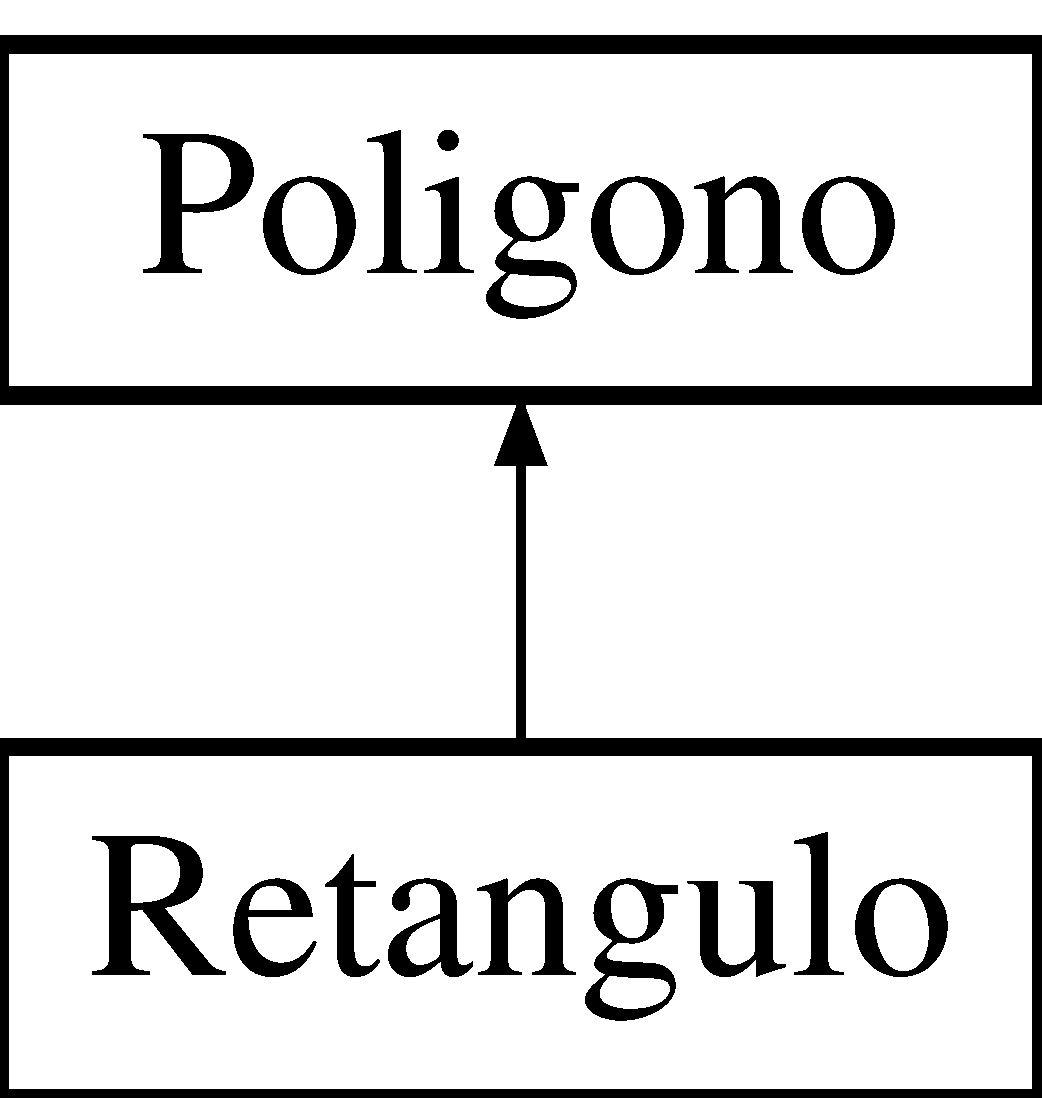
\includegraphics[height=2.000000cm]{class_poligono}
\end{center}
\end{figure}
\subsection*{Public Member Functions}
\begin{DoxyCompactItemize}
\item 
\mbox{\Hypertarget{class_poligono_a9311a9a1496878c09c8508b3636e2870}\label{class_poligono_a9311a9a1496878c09c8508b3636e2870}} 
\mbox{\hyperlink{class_poligono_a9311a9a1496878c09c8508b3636e2870}{Poligono}} ()
\begin{DoxyCompactList}\small\item\em \mbox{\hyperlink{class_poligono}{Poligono}} é o construtor da classe. \end{DoxyCompactList}\item 
void \mbox{\hyperlink{class_poligono_a3fb101362b44fb9682e33cba0d3cd5ed}{insert}} (\mbox{\hyperlink{class_point}{Point}} vertice1)
\begin{DoxyCompactList}\small\item\em insert é uma função da classe que serve para inserir um ponto do poligono. \end{DoxyCompactList}\item 
int \mbox{\hyperlink{class_poligono_a81116a54985e6e897bd785268ba35a6e}{recupera}} (void)
\begin{DoxyCompactList}\small\item\em recupera é uma função da classe que serve para recuperar o numero de vertices do poligono. \end{DoxyCompactList}\item 
float \mbox{\hyperlink{class_poligono_a9b7cb6c339f78a5b9432494d8f94816c}{area}} (void)
\begin{DoxyCompactList}\small\item\em area é uma função da classe que serve para calcular a area do poligono convexo. \end{DoxyCompactList}\item 
void \mbox{\hyperlink{class_poligono_a48b40bd2284a5c7ee5253f2070052046}{transladar}} (float a, float b)
\begin{DoxyCompactList}\small\item\em transladar é uma função da classe que serve para translatar todos os pontos do poligono. \end{DoxyCompactList}\item 
void \mbox{\hyperlink{class_poligono_a2d58ed88cb9be91bb0047984dc1dd054}{rotacionar}} (float teta, \mbox{\hyperlink{class_point}{Point}} p1)
\begin{DoxyCompactList}\small\item\em rotacionar é uma classe que serve para rotacionar o poligono a partir de um valor em radianos de angulo teta. \end{DoxyCompactList}\item 
\mbox{\Hypertarget{class_poligono_af61200b446e9fda58a42355eec49d433}\label{class_poligono_af61200b446e9fda58a42355eec49d433}} 
void \mbox{\hyperlink{class_poligono_af61200b446e9fda58a42355eec49d433}{imprimir}} (void)
\begin{DoxyCompactList}\small\item\em imprime é uma função da classe que serve para imprimir o conjunto de pontos do poligono na tela. \end{DoxyCompactList}\end{DoxyCompactItemize}
\subsection*{Protected Attributes}
\begin{DoxyCompactItemize}
\item 
\mbox{\Hypertarget{class_poligono_a18179d267bdf366f6bb00a4e1b16f1d7}\label{class_poligono_a18179d267bdf366f6bb00a4e1b16f1d7}} 
\mbox{\hyperlink{class_point}{Point}} {\bfseries vertices} \mbox{[}100\mbox{]}
\item 
\mbox{\Hypertarget{class_poligono_af9259ab305f65ba3ac2fa256d72cc047}\label{class_poligono_af9259ab305f65ba3ac2fa256d72cc047}} 
int {\bfseries nv}
\end{DoxyCompactItemize}


\subsection{Detailed Description}
The Pologono class serve para realizar e manipular pontos de um poligono convexo. 

\subsection{Member Function Documentation}
\mbox{\Hypertarget{class_poligono_a9b7cb6c339f78a5b9432494d8f94816c}\label{class_poligono_a9b7cb6c339f78a5b9432494d8f94816c}} 
\index{Poligono@{Poligono}!area@{area}}
\index{area@{area}!Poligono@{Poligono}}
\subsubsection{\texorpdfstring{area()}{area()}}
{\footnotesize\ttfamily float Poligono\+::area (\begin{DoxyParamCaption}\item[{void}]{ }\end{DoxyParamCaption})}



area é uma função da classe que serve para calcular a area do poligono convexo. 

\begin{DoxyReturn}{Returns}
o valor da área calculada. 
\end{DoxyReturn}
\mbox{\Hypertarget{class_poligono_a3fb101362b44fb9682e33cba0d3cd5ed}\label{class_poligono_a3fb101362b44fb9682e33cba0d3cd5ed}} 
\index{Poligono@{Poligono}!insert@{insert}}
\index{insert@{insert}!Poligono@{Poligono}}
\subsubsection{\texorpdfstring{insert()}{insert()}}
{\footnotesize\ttfamily void Poligono\+::insert (\begin{DoxyParamCaption}\item[{\mbox{\hyperlink{class_point}{Point}}}]{vertice1 }\end{DoxyParamCaption})}



insert é uma função da classe que serve para inserir um ponto do poligono. 


\begin{DoxyParams}{Parameters}
{\em vertice1} & é o ponto a ser enserido. \\
\hline
\end{DoxyParams}
\mbox{\Hypertarget{class_poligono_a81116a54985e6e897bd785268ba35a6e}\label{class_poligono_a81116a54985e6e897bd785268ba35a6e}} 
\index{Poligono@{Poligono}!recupera@{recupera}}
\index{recupera@{recupera}!Poligono@{Poligono}}
\subsubsection{\texorpdfstring{recupera()}{recupera()}}
{\footnotesize\ttfamily int Poligono\+::recupera (\begin{DoxyParamCaption}\item[{void}]{ }\end{DoxyParamCaption})}



recupera é uma função da classe que serve para recuperar o numero de vertices do poligono. 

\begin{DoxyReturn}{Returns}
número de vertices. 
\end{DoxyReturn}
\mbox{\Hypertarget{class_poligono_a2d58ed88cb9be91bb0047984dc1dd054}\label{class_poligono_a2d58ed88cb9be91bb0047984dc1dd054}} 
\index{Poligono@{Poligono}!rotacionar@{rotacionar}}
\index{rotacionar@{rotacionar}!Poligono@{Poligono}}
\subsubsection{\texorpdfstring{rotacionar()}{rotacionar()}}
{\footnotesize\ttfamily void Poligono\+::rotacionar (\begin{DoxyParamCaption}\item[{float}]{teta,  }\item[{\mbox{\hyperlink{class_point}{Point}}}]{p1 }\end{DoxyParamCaption})}



rotacionar é uma classe que serve para rotacionar o poligono a partir de um valor em radianos de angulo teta. 


\begin{DoxyParams}{Parameters}
{\em teta} & o valor em radiano para a rotação. \\
\hline
{\em p1} & ponto base de rotação do poligono. \\
\hline
\end{DoxyParams}
\mbox{\Hypertarget{class_poligono_a48b40bd2284a5c7ee5253f2070052046}\label{class_poligono_a48b40bd2284a5c7ee5253f2070052046}} 
\index{Poligono@{Poligono}!transladar@{transladar}}
\index{transladar@{transladar}!Poligono@{Poligono}}
\subsubsection{\texorpdfstring{transladar()}{transladar()}}
{\footnotesize\ttfamily void Poligono\+::transladar (\begin{DoxyParamCaption}\item[{float}]{a,  }\item[{float}]{b }\end{DoxyParamCaption})}



transladar é uma função da classe que serve para translatar todos os pontos do poligono. 


\begin{DoxyParams}{Parameters}
{\em a} & quantidade a ser transladada no eixo x. \\
\hline
{\em b} & quantidade a ser transladada no eixo y. \\
\hline
\end{DoxyParams}


The documentation for this class was generated from the following files\+:\begin{DoxyCompactItemize}
\item 
poligono.\+h\item 
poligono.\+cpp\end{DoxyCompactItemize}

\hypertarget{class_retangulo}{}\section{Retangulo Class Reference}
\label{class_retangulo}\index{Retangulo@{Retangulo}}


The \mbox{\hyperlink{class_retangulo}{Retangulo}} class cria e manipula poligonos do tipo retangular.  




{\ttfamily \#include $<$retangulo.\+h$>$}

Inheritance diagram for Retangulo\+:\begin{figure}[H]
\begin{center}
\leavevmode
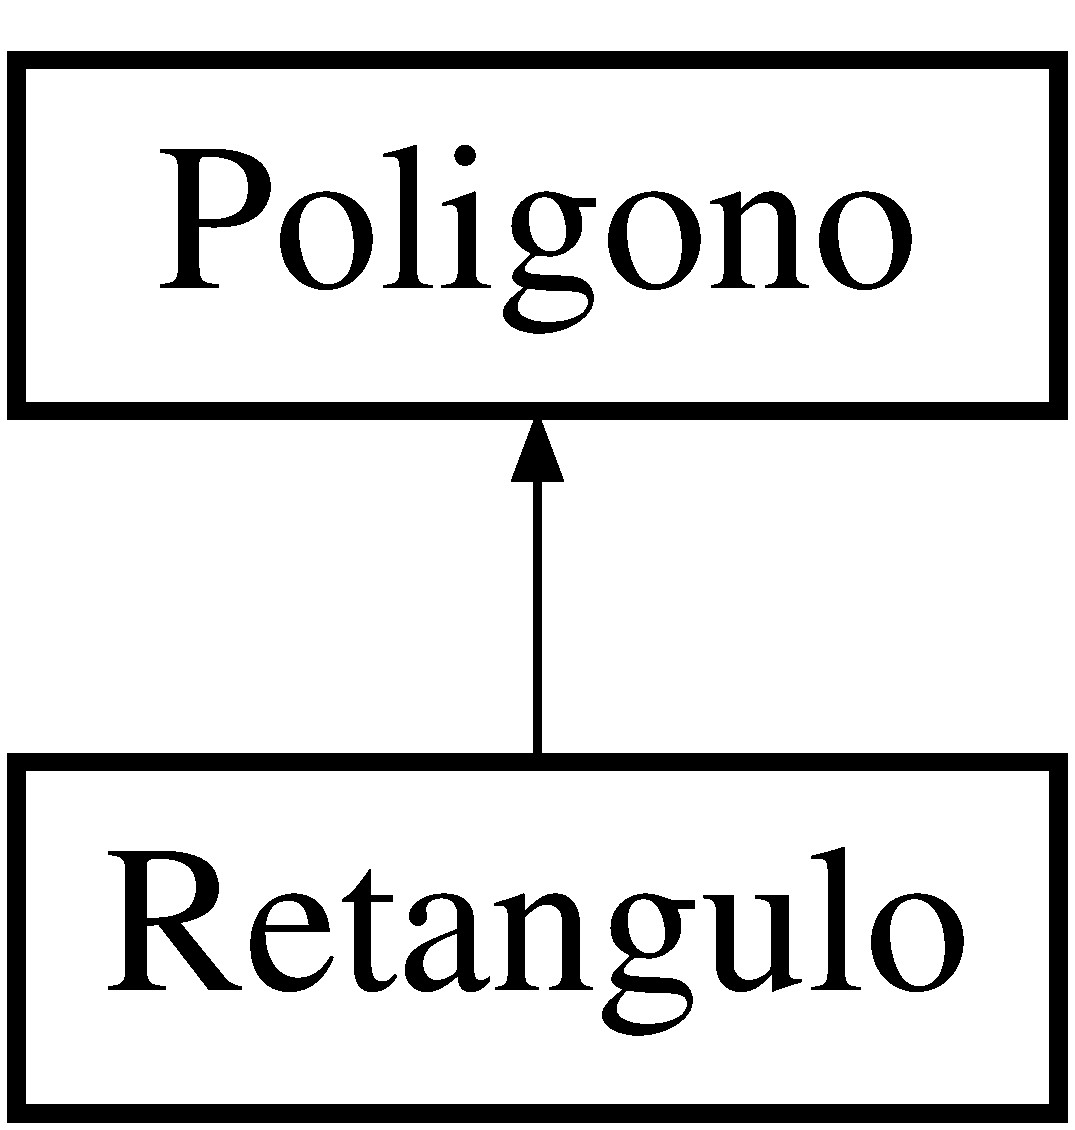
\includegraphics[height=2.000000cm]{db/df7/class_retangulo}
\end{center}
\end{figure}
\subsection*{Public Member Functions}
\begin{DoxyCompactItemize}
\item 
\mbox{\hyperlink{class_retangulo_acca1dd211eefc8dc04658c943c0d1122}{Retangulo}} (float x, float y, float largura, float altura)
\begin{DoxyCompactList}\small\item\em \mbox{\hyperlink{class_retangulo}{Retangulo}} é o construtor da classe. \end{DoxyCompactList}\end{DoxyCompactItemize}
\subsection*{Additional Inherited Members}


\subsection{Detailed Description}
The \mbox{\hyperlink{class_retangulo}{Retangulo}} class cria e manipula poligonos do tipo retangular. 

\subsection{Constructor \& Destructor Documentation}
\mbox{\Hypertarget{class_retangulo_acca1dd211eefc8dc04658c943c0d1122}\label{class_retangulo_acca1dd211eefc8dc04658c943c0d1122}} 
\index{Retangulo@{Retangulo}!Retangulo@{Retangulo}}
\index{Retangulo@{Retangulo}!Retangulo@{Retangulo}}
\subsubsection{\texorpdfstring{Retangulo()}{Retangulo()}}
{\footnotesize\ttfamily Retangulo\+::\+Retangulo (\begin{DoxyParamCaption}\item[{float}]{x,  }\item[{float}]{y,  }\item[{float}]{largura,  }\item[{float}]{altura }\end{DoxyParamCaption})}



\mbox{\hyperlink{class_retangulo}{Retangulo}} é o construtor da classe. 


\begin{DoxyParams}{Parameters}
{\em x} & é a posição no eixo x do ponto inicial do retangulo. \\
\hline
{\em y} & é a posição no eixo y do ponto inicial do retangulo. \\
\hline
{\em largura} & é a distância entre os pontos da base do retangulo no eixo x. \\
\hline
{\em altura} & é a distância entre os pontos da lateral do retangulo no eixo y. \\
\hline
\end{DoxyParams}


The documentation for this class was generated from the following files\+:\begin{DoxyCompactItemize}
\item 
retangulo.\+h\item 
retangulo.\+cpp\end{DoxyCompactItemize}

%--- End generated contents ---

% Index
\backmatter
\newpage
\phantomsection
\clearemptydoublepage
\addcontentsline{toc}{chapter}{Index}
\printindex

\end{document}
